Software design goes here.

\section{Neural Networks}

\begin{figure}
	\centering
	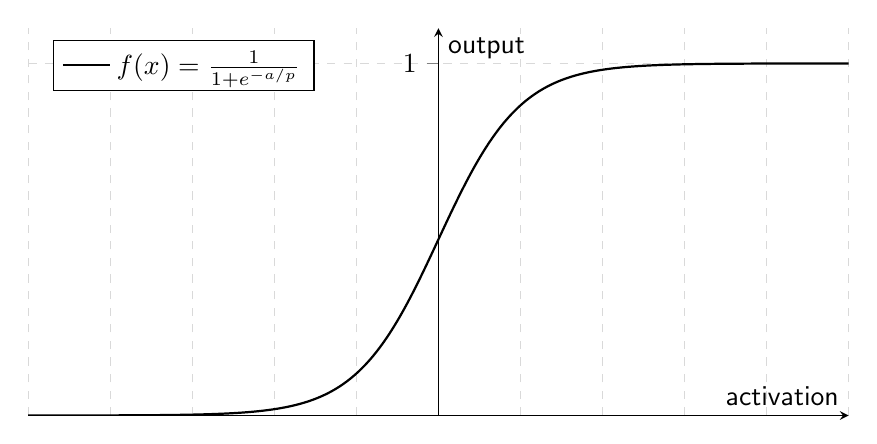
\begin{tikzpicture}[font=\sffamily]
    \begin{axis}[
    	legend pos=north west,
        axis x line=middle,
        axis y line=middle,
        grid = major,
        width=12cm,
        height=6.5cm,
        grid style={dashed, gray!30},
        xmin=-1,xmax= 1,ymin= 0,ymax= 1.1,
        xlabel=activation,ylabel=output,
        tick align=outside,
        ytick={1},
        xmajorticks=false,
        enlargelimits=false]
      \addplot[domain=-1:1,black,thick,samples=500] {1/(1+exp(-10*x))}; 
      \addlegendentry{$f(x)=\frac{1}{1+e^{-a/p}}$}
    \end{axis} 
\end{tikzpicture}
	\caption{Sigmoid Function Graph}
\end{figure}

\begin{figure}[h]
	\centering
	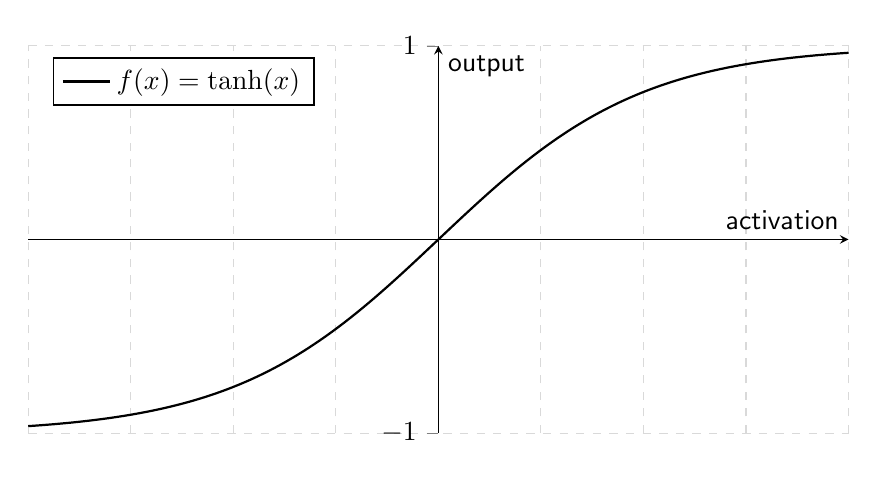
\begin{tikzpicture}[font=\sffamily]
    \begin{axis}[
    	legend pos=north west,
        axis x line=middle,
        axis y line=middle,
        grid = major,
        width=12cm,
        height=6.5cm,
        grid style={dashed, gray!30},
        xmin=-2,xmax= 2,ymin= -1,ymax= 1,
        xlabel=activation,ylabel=output,
        tick align=outside,
        ytick={-1,1},
        xmajorticks=false,
        enlargelimits=false]
      \addplot[domain=-2:2,black,thick,samples=500] {tanh(x)}; 
      \addlegendentry{$f(x)=\tanh(x)$}
    \end{axis} 
\end{tikzpicture}
	\caption{Hyperbolic Tangent Function Graph}
\end{figure}

\begin{figure}[h]
	\centering
	\def\layersep{2.5cm}
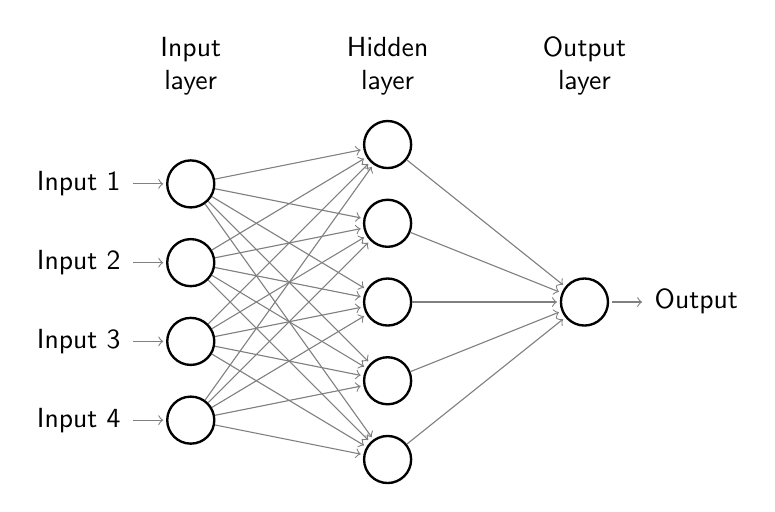
\begin{tikzpicture}[shorten >=1pt,->,draw=black!50, node distance=\layersep,font=\sffamily]
    \tikzstyle{every pin edge}=[<-,shorten <=1pt]
    \tikzstyle{neuron}=[circle,line width=0.3mm,draw=black,minimum size=17pt,inner sep=0pt]
    \tikzstyle{annot} = [text width=4em, text centered]

    \foreach \name / \y in {1,...,4}
        \node[neuron, pin=left:Input \y] (I-\name) at (0,-\y) {};

    \foreach \name / \y in {1,...,5}
        \path[yshift=0.5cm]
            node[neuron] (H-\name) at (\layersep,-\y cm) {};

    \node[neuron,pin={[pin edge={->}]right:Output}, right of=H-3] (O) {};

    \foreach \source in {1,...,4}
        \foreach \dest in {1,...,5}
            \path (I-\source) edge (H-\dest);

    \foreach \source in {1,...,5}
        \path (H-\source) edge (O);

    %\draw[->] (5,-2.9) -- (5,-5) -- (1,-5) -- (1,-4.5);
    %\node (1,-4.5) {Error back propagation}

    \node[annot,above of=H-1, node distance=1cm] (hl) {Hidden layer};
    \node[annot,left of=hl] {Input layer};
    \node[annot,right of=hl] {Output layer};
\end{tikzpicture}
	\caption{Single Output Feedforward Network}
\end{figure}

%example psuedocode (http://mirrors.ibiblio.org/CTAN/macros/latex/contrib/algorithmicx/algorithmicx.pdf for reference)
\begin{algorithm}[!ht]
	\caption{FizzBuzz Algorithm}
	\begin{algorithmic}[1]
		\For{each integer $i$ 1 to 100}
			\If{$15 \mid i$}
				\State print ``FizzBuzz''
			\ElsIf{$3 \mid i$}
				\State print ``Fizz''
			\ElsIf{$5 \mid i$}
				\State print ``Buzz''
			\Else
				\State print $i$
			\EndIf
		\EndFor
	\end{algorithmic}
\end{algorithm}

\section{Reinforcement Learning}

\section{Convergent Wire Fitted Neural Network Q-Learning}
